\documentclass{article}
\usepackage[utf8]{inputenc}
\usepackage{float}

\title{TP2 - Consumo de Drogas}
\author{Arthur de Assis Silva e Luciana Barreto Lima}
\date{05 de dezembro de 2018}

\usepackage{natbib}
\usepackage{graphicx}
\usepackage{url}
\usepackage[portuguese, ruled, linesnumbered]{algorithm2e}
\usepackage{pdfpages}
\usepackage[figuresleft]{rotating}

\begin{document}

\maketitle

\section{Objetivo}

Sabe-se que existem vários perfis de pessoas que fazem uso de drogas. Esse perfil varia, principalmente, de acordo com o tipo de droga, pois existem as drogas lícitas, ilícitas, mais fracas e mais fortes. O objetivo desse trabalho prático é identificar em quantos clusters os usuários de drogas se agrupam e qual são as principais características de cada um dos grupos.

Com base nessas informações, é possível entender as principais motivações para o consumo de drogas para cada grupo e atuar na prevenção de forma mais efetiva e até mesmo identificar a melhor forma de abordar um usuário para um tratamento.  

\section{Contexto}

No mundo inteiro, o consumo de drogas é um dos principais problemas de saúde pública. O uso da maior parte das drogas provoca, em um primeiro momento, efeitos muito positivos como sensação de bem-estar, felicidade e coragem. No entanto, seus efeitos a longo prazo podem ser muito graves, especialmente quando utilizadas por muito tempo.

O uso de drogas pode provocar alterações sérias no funcionamento do coração, do fígado, pulmões e até mesmo do cérebro, sendo muito prejudicial à saúde e podendo levar à morte.

Além disso, uma boa parte das drogas causa vício e, por isso, o corpo vai precisando de uma dose cada vez superior para conseguir obter os mesmos resultados positivos, o que aumenta muito o risco de morte por overdose.

\section{Base de dados}\label{secao_base_dados}

A base de dados a ser utilizada no trabalho foi baixada por meio do link \url{<http://archive.ics.uci.edu/ml/datasets/Drug+consumption%28quantified%29>}, O Banco de dados contém registros para 1885 respondentes e atributos como medições de personalidade, escolaridade, idade, sexo, país de residência e etnia. Todos os atributos de entrada são originalmente categóricos e são quantificados. Além disso, os participantes foram questionados sobre o uso de 18 drogas legais e ilegais e para cada uma delas eles tiveram que selecionar uma das respostas: nunca usaram a droga, a usaram mais de uma década atrás, ou na última década, ano, mês, semana ou dia.

\section{Metodologia}

Este trabalho prático foi implementado em Python para o pré-processamento da base de dados e avaliação dos modelos e no Lemonade para a aplicação dos algoritmos de agrupamento. O código do Fluxo de Execução deste trabalho no Lemonade é \#304.  

Existem inúmeros algoritmos de clusterização. No presente trabalho vamos trabalhar com dois dos mais populares: K-Means e o EM - Gaussian Mixture.

\subsection{Pré-processamento da base de dados}

Para servir como input para os algoritmos de agrupamento, a base de dados precisou passar por alguns tratamentos. De forma geral, a base de dados é bem consistente, não possui dados faltantes e a maioria das variáveis são numéricas. Apenas um conjunto de features estava como string na base de dados e foi aplicada uma codificação, para transformá-las em categóricas ordinais, pois possuem uma ordenação lógica.

\subsection{Algoritmos de agrupamento}

O algoritmo K-means é um algoritmo de agrupamento iterativo que classifica instâncias em K de grupos, sendo que o número de cluster deve ser previamente definido. 

O K-means tem como função de classificação a distância entre os pontos na base de dados ao centro dos grupos (centroide). A solução final é a que minimiza a soma das distâncias entre cada ponto e o seu centroide. 

O algoritmo EM - Gaussian Mixture é baseado em modelos quem tentam otimizar o ajuste entre os dados fornecidos e algum modelo matemático, no caso a distribuição normal multivariada. Pode ser considerado uma extensão do K-means, o qual atribui objetos ao grupo que é mais similar, com base na média do grupo. Em vez de atribuir cada objeto a um grupo exclusivo, o EM atribui cada objeto
para os grupos de acordo com um peso representando a probabilidade do objeto pertencer a tais grupos. Dessa forma, não existem limites estritos entre os grupos. 

Modelos de misturas são mais gerais do que K-means porque podem usar distribuições de diversos tipos, podem encontrar grupos de tamanhos diferentes, densidades diferentes e formatos elípticos. No entanto, não funcionam tão bem a medida que o número de features cresce muito.

\subsection{Escolha do número ótimo de grupos}

Ambos os algoritmos escolhidos precisam receber como parâmetro a quantidade de cluster, que deve ser definida previamente. Um processo muito usado para definir o número ótimo de grupos é o \textit{Elbow Method }, que consiste em executar o algoritmo K-means para vários números de cluster, armazenar a medida WSS, plotar o gráfico com o WSS para cada quantidade de grupos e identificar o ponto que minimiza o WSS para o número menor de grupos, formando um cotovelo (Elbow). 

A medida WSS é a soma dos quadrados da diferença entre os pontos e seus respectivos centroides, também chamado de inércia.

\subsection{Medidas de qualidade do agrupamento}

Para mensurar a qualidade dos agrupamentos vamos usar as medidas Silhouette Coefficient e Calinski-Harabaz Index.

O Silhouette Coefficient, proposto por \cite{rousseeuw:1987} , é bastante usado quando o rótulo verdadeiro não é conhecido e a avaliação deve ser realizada usando o próprio modelo. É calculado usando a distância intra-cluster média e a distância média do cluster mais próximo para cada amostra.
Essa métrica varia entre -1 e 1, um valor próximo de 1 indica que o agrupamento está bem definido, se for próximo de 0 significa que os grupos estão sobrepostos e se for próximo à -1, mostra que o agrupamento não ficou bem definido.

Já o Calinski-Harabaz Index, proposto por \cite{calinski1974}, é também conhecido como o Critério de Variação, a pontuação é definida como a razão entre a dispersão dentro do cluster e a dispersão entre clusters. A pontuação é maior quando os clusters são densos e bem separados, o que se relaciona com um conceito padrão de um cluster.

\section{Resultados experimentais}

Para escolher a quantidade de clusters ótima para ser usada como parâmetro para os algoritmos, utilizamos um conjunto de 20 valores e analisamos a medida WSS gerada por cada um destes valores. O figura \ref{elbow} mostra os valores de WSS obtidos para os diferentes números de clusters.

\begin{figure}[H]
\centering
    \includegraphics[width=80mm]{resultados/elbow}
\caption{Inércias geradas pelos diferentes tamanhos de k}
\label{elbow}
\end{figure}

Analisando a figura \ref{elbow} são encontrados dois valores que minimizam o WSS (3 e 7). Para auxiliar na escolha do melhor valor foram analisadas as métricas Calinski-Harabaz Index e Silhouette Coefficient. A figura \ref{metricas} apresenta os resultados obtidos por cada métrica em cada algoritmo.

\begin{figure}[H]
\begin{tabular}{cc}
    \includegraphics[width=65mm]{resultados/Calinski} & \includegraphics[width=65mm]{resultados/Silhouette}\\
    (a) Calinski-Harabaz Index & (b) Silhouette Coefficient \\[6pt]
\end{tabular}
\caption{Métricas de qualidade dos algoritmos}
\label{metricas}
\end{figure}

Após analisar a figura \ref{metricas} foi escolhido a quantidade de três clusters para o algoritmo K-means, pois, esta quantidade fornece clusters mais densos e mais separados.
 
\begin{figure}[H]
\begin{tabular}{cc}
    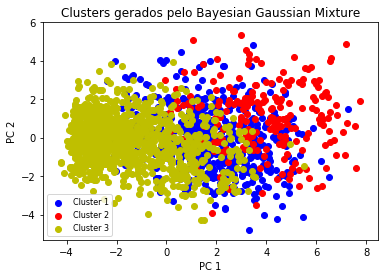
\includegraphics[width=65mm]{resultados/clusters_gmm} & 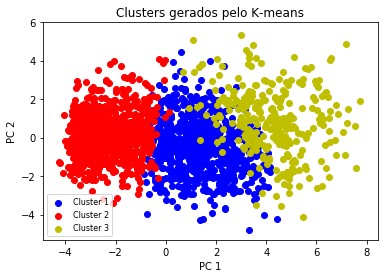
\includegraphics[width=65mm]{resultados/clusters_kmeans}\\
    (a) GMM & (b) K-means \\[6pt]
\end{tabular}
\caption{Clusters gerados pelos modelos GMM e K-means}
\label{clusters}
\end{figure}

As figuras \ref{metricas} e \ref{clusters} mostram que para um $k$ igual a 3, o algoritmo k-means apresenta resultados melhores em relação ao algortimo GMM, já que possui grupos mais homogêneos internamente e bem delimitados. Após definir o tamanho de $k$ e obter qual dos três clusters cada observação pertence, foi executado uma \textit{Random Forest} \citep{Breiman2001} sobre o \textit{dataset} tendo como target os clusters gerados pelo K-means. A figura \ref{feature_importance} apresenta a importância das features para a classificação das observações em cada cluster segundo o \textit{Random Forest}. Ela mostra as características mais consideradas no processo de classificação, sendo o consumo de cogumelos e maconha as características mais importantes e o uso de cafeína e o sexo do indivíduo as menos relevantes.

\begin{figure}[H]
\centering
    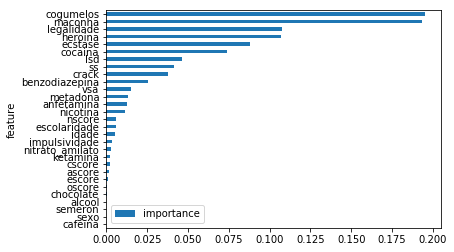
\includegraphics[width=120mm]{resultados/feature_importance_original}
\caption{Importância das features para a classificação dos clusters}
\label{feature_importance}
\end{figure}

Para analisar a Figura \ref{arvore} e entender quais são as características predominantes dos usuários de drogas presentes em cada cluster, a tabela \ref{categorias} apresenta o significado das categorias usadas para representar a distribuição do consumo drogas. 

\begin{table}[H]
\centering
\begin{tabular}{|c|l|}
\hline
Categoria & Significado        \\ \hline
0                       & Nunca usou         \\ \hline
1                       & Mais de uma década \\ \hline
2                       & Última década      \\ \hline
3                       & Ano passado        \\ \hline
4                       & Mês passado        \\ \hline
5                       & Semana passada     \\ \hline
6                       & Ontem              \\ \hline
\end{tabular}
\caption{Significados das categorias para representar as features.}
\label{categorias}
\end{table}

O percentual de elementos em cada cluster gerado pelo K-means foi de 47\%, 15\% e 38\% nos Clusters 1, 2 e 3, respectivamente. A árvore de decisão apresentada pela Figura \ref{arvore} mostra quais conjuntos de características são utilizadas para definir em qual cluster cada elemento será agrupado. Nela é possível identificar que as características dos componentes do Cluster 1 (azul) são pessoas que tiveram um contato há mais de uma década com drogas como cogumelos, maconha ou heroína ou teve contato há menos de um ano com maconha e menos de uma década com ecstasy. O Cluster 2 (amarelo) é composto por usuários que usaram cogumelos há menos de uma década, usaram maconha no último mês e usaram cocaína há mais de um ano. Por último, o Cluster 3 (vermelho) é composto por usuários que usaram cogumelos e crack na última década, cocaína no ano passado e heroína há mais de uma década. 

\newpage
\begin{figure}[H]
\centering
    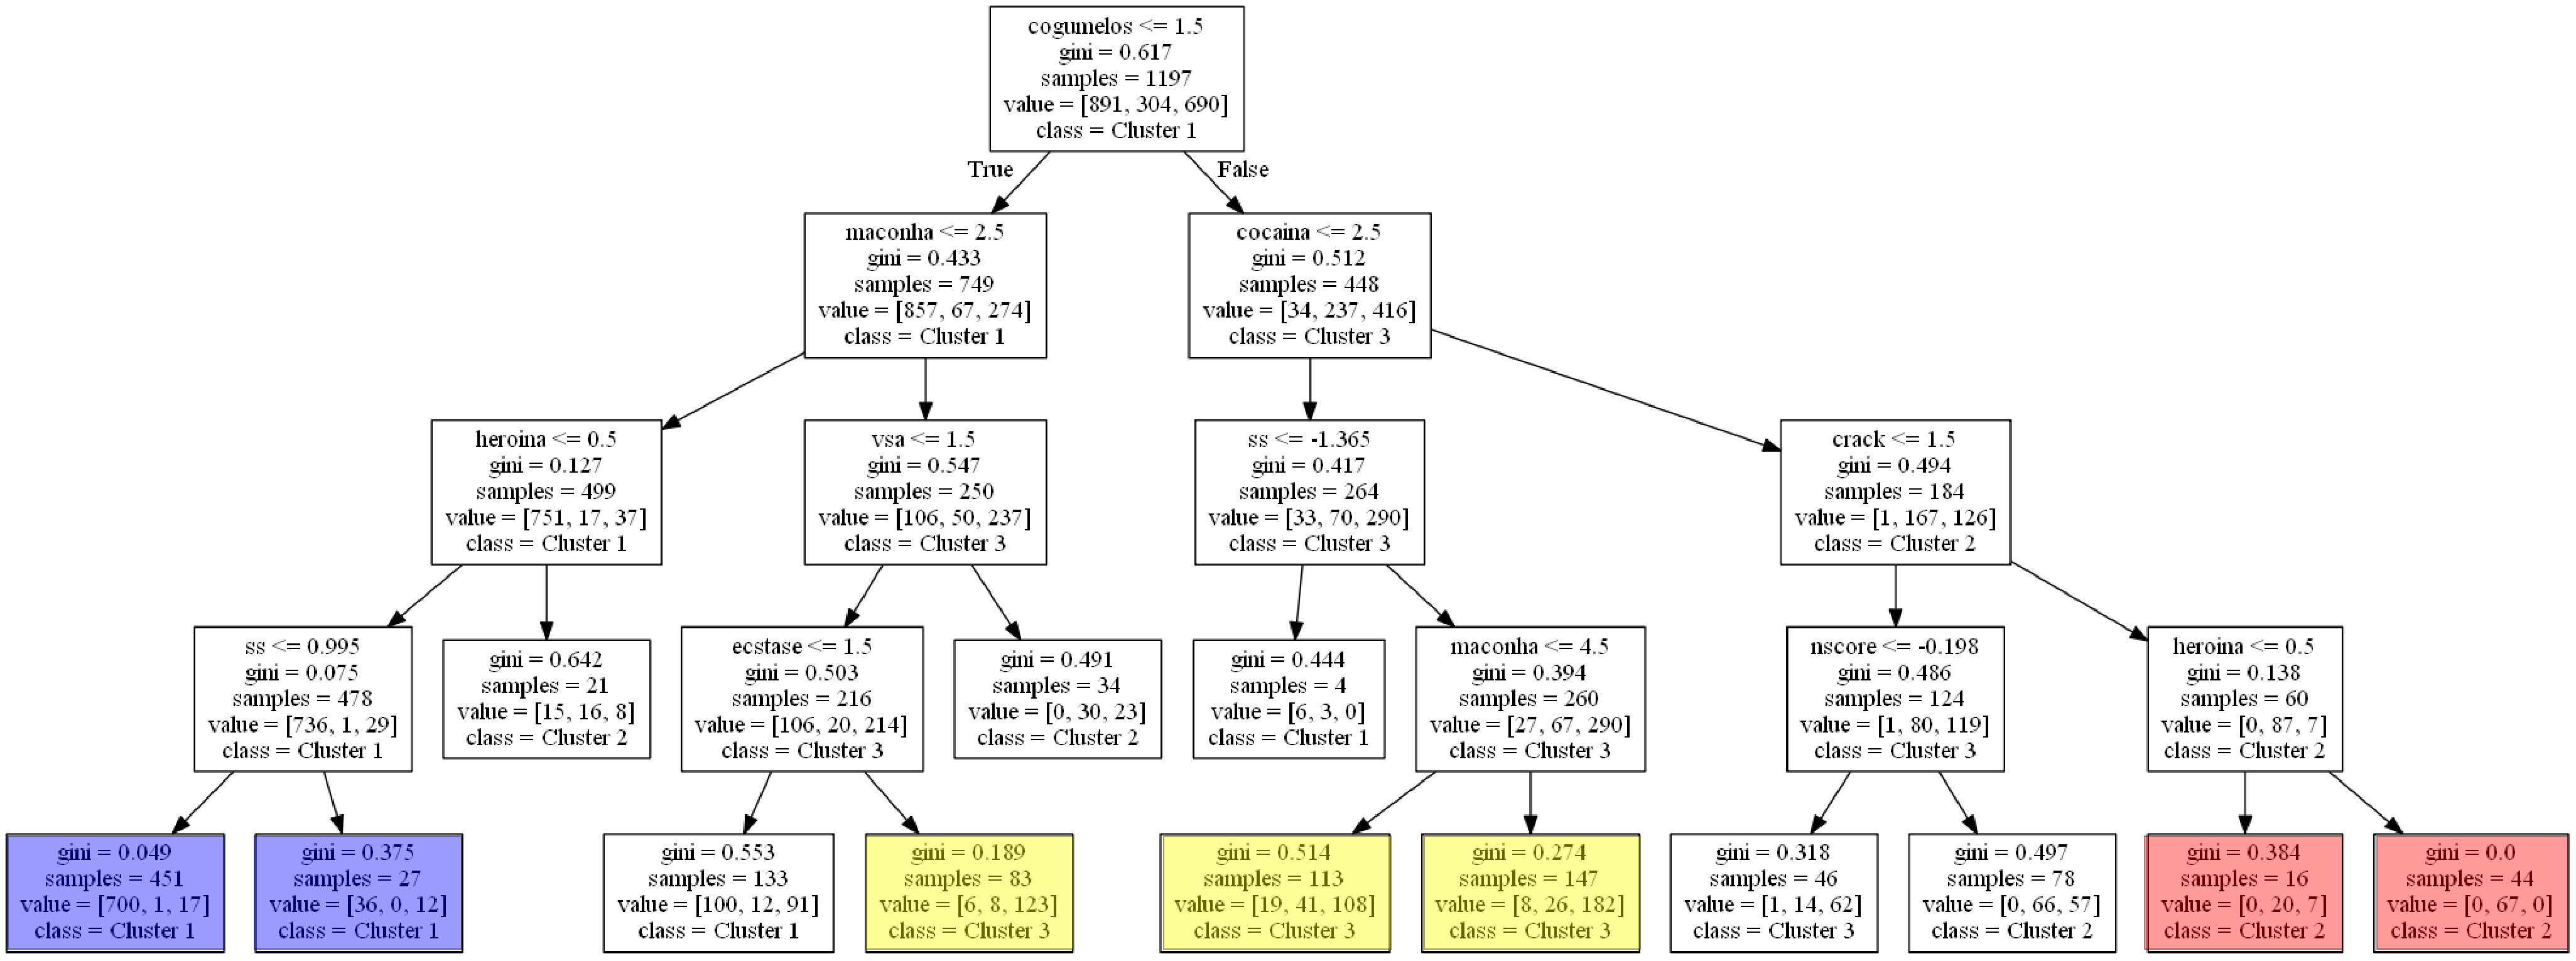
\includegraphics[scale=0.32, angle=270]{resultados/Arvore.pdf}
    \caption{Árvore de decisão}
\label{arvore}
\end{figure}
 
\section{Conclusões}
 
O trabalho apresentou uma comparação entre dois algoritmos de clusterização, o algoritmo K-means e o GMM. A partir de análises realizadas foi escolhido o K-means devido à qualidade da solução gerada. Ele foi capaz de gerar para o conjunto de dados analisados, clusters mais densos e mais separados. Foi utilizada uma árvore de decisão para analisar as características predominantes nos componentes de cada agrupamento e quais características (features) possuem uma importância maior no processos de construção dos clusters.

\bibliographystyle{apalike}
\bibliography{references}

\end{document}
